\section{Custom CNN Training and Evaluation}
\subsection{Training Setup}
Both custom models are initialized afresh and trained for 25 epochs using the
selected optimizer Adam at learning rate 0.001, batch size 128 and cross-entropy
loss. Thus both exceed the required minimum of 20 epochs. Computation uses
32-bit floating point (FP32) on an NVIDIA GeForce RTX 5060 Laptop GPU. Deterministic algorithms and
seed 3150 are enabled. The best validation-accuracy checkpoint, with validation
loss breaking ties, is retained. There is no early stopping. The first ten
epochs of the final Model B run exactly reproduce its Adam pilot losses and
accuracies. One reusable training loop handles the custom and pretrained
models, with configurable epochs, batch size and optimizer, CUDA support and
CPU fallback. Python 3.14.5, PyTorch 2.13.0+cu130 and torchvision 0.28.0+cu130
are recorded in each run's JSON. CSV histories contain every epoch's losses,
accuracies, stage and elapsed time. Checkpoints store the validation-selected
weights, not the final epoch by default.
\subsection{Training Curves}
Figures~\ref{fig:model_a_curves} and~\ref{fig:model_b_curves} show the complete
training histories. Both training losses decrease overall, while validation
losses fluctuate. The gap between training and validation performance near
the end suggests that continued fitting of the training set does not reliably
improve held-out performance.
\begin{figure}[H]\centering
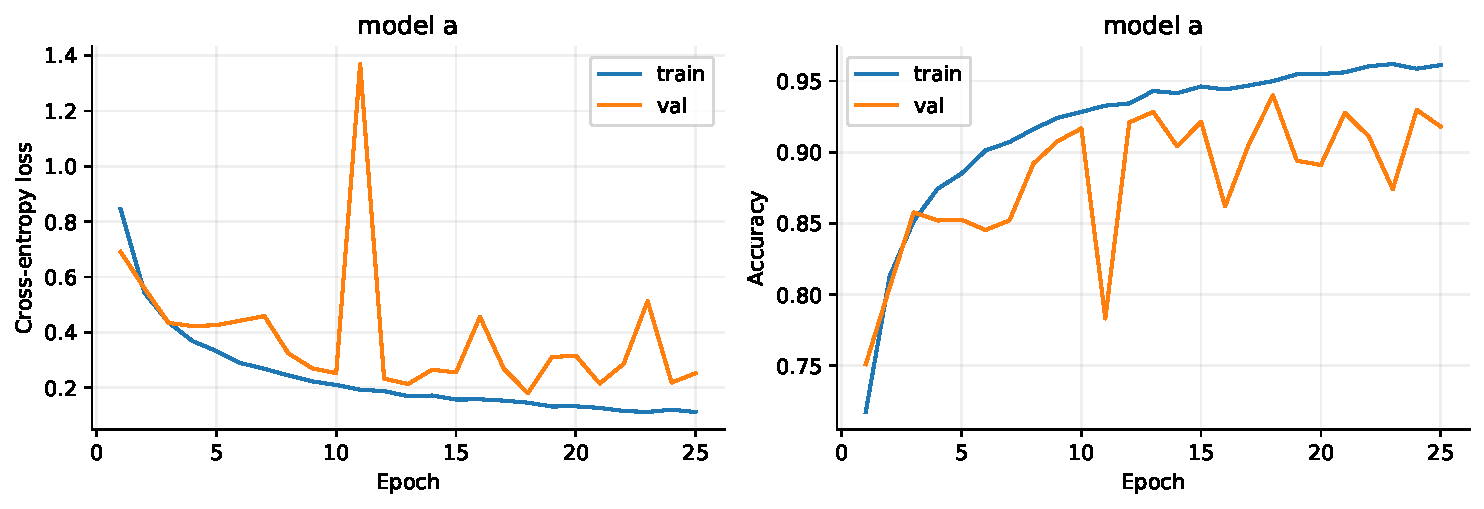
\includegraphics[width=0.96\textwidth]{figures/model_a_curves.pdf}
\caption{Model A training and validation history.}
\label{fig:model_a_curves}
\end{figure}
Model A selects epoch \ABestEpoch{} with \ABestVal\% validation accuracy.
Final training/validation accuracies are \AFinalTrain\%/\AFinalVal\%.
Its largest epoch-to-epoch validation drop is \AWorstDrop{} percentage points
at epoch 11, followed by recovery. This is a temporary instability in the
observed validation trajectory; the experiment does not identify its cause.
\begin{figure}[H]\centering
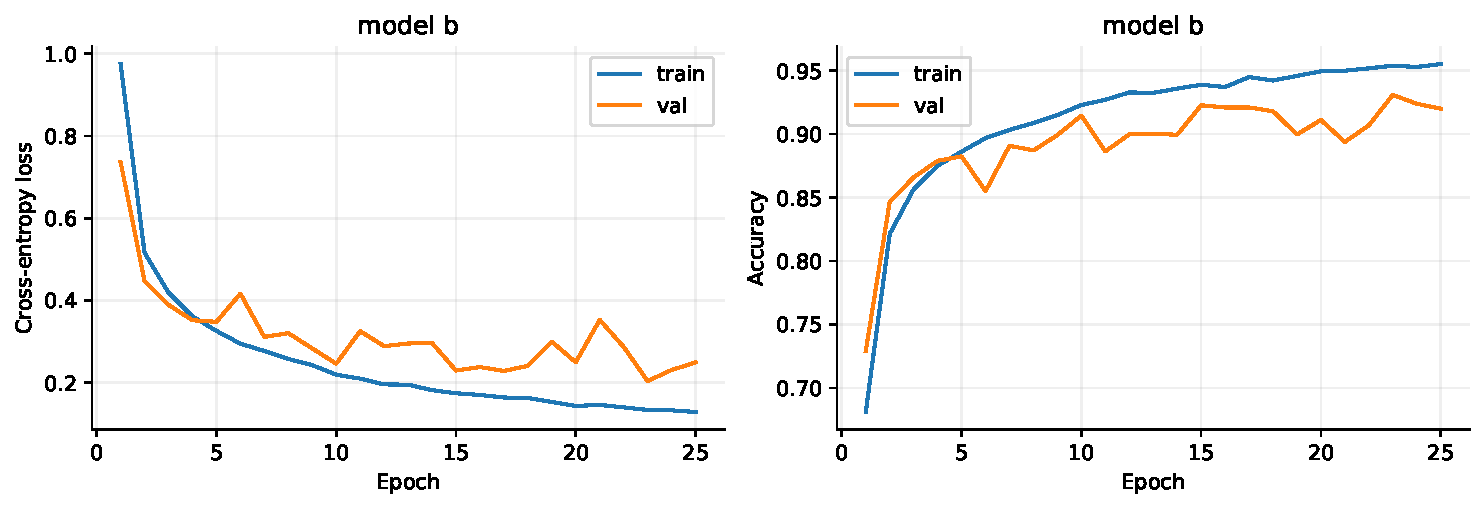
\includegraphics[width=0.96\textwidth]{figures/model_b_curves.pdf}
\caption{Model B training and validation history.}
\label{fig:model_b_curves}
\end{figure}
Model B selects epoch \BBestEpoch{} with \BBestVal\% validation accuracy.
Final training/validation accuracies are \BFinalTrain\%/\BFinalVal\%.
Its largest epoch-to-epoch validation drop is \BWorstDrop{} percentage points
at epoch 11, smaller than Model A's largest drop. However, neither run gives
a monotonic validation improvement, which supports retaining the best
validation checkpoint rather than using the last epoch automatically.
\subsection{Test Results}
Accuracy is the fraction of correct predictions. Precision and recall are
unweighted macro averages over all ten classes; undefined class precision is
set to zero. Each selected checkpoint is evaluated on the untouched test set.
For class $c$, let $TP_c$, $FP_c$ and $FN_c$ denote true positives, false
positives and false negatives. With $C=10$ classes and $N=4050$ test images,
\begin{equation}
\begin{aligned}
\mathrm{Accuracy}&=\frac{\sum_c TP_c}{N},\\
\mathrm{MacroPrecision}&=\frac{1}{C}\sum_{c=1}^{C}\frac{TP_c}{TP_c+FP_c},\\
\mathrm{MacroRecall}&=\frac{1}{C}\sum_{c=1}^{C}\frac{TP_c}{TP_c+FN_c}.
\end{aligned}\label{eq:metrics}
\end{equation}
The scikit-learn calculations in Table~\ref{tab:custom_accuracy} follow
Equation~\eqref{eq:metrics}. Model A is slightly higher on all three aggregate
metrics, but its accuracy advantage corresponds to only \CustomCorrectGap{}
additional correct predictions on this test set. This is a small observed
difference, not evidence of a consistent advantage over repeated runs.
% Generated from saved experiment evidence; do not edit values.
\begin{table}[H]\centering\small
\caption{Held-out test metrics for custom models; P is precision and R is recall.}\label{tab:custom_accuracy}
\begin{tabular}{lrrr}
\toprule
Model & Accuracy (\%) & Macro P (\%) & Macro R (\%) \\ \midrule
Model A & 94.30 & 94.25 & 94.26 \\
Model B & 94.15 & 94.00 & 93.88 \\
\bottomrule
\end{tabular}
\end{table}

\subsection{Confusion Matrices}
Figures~\ref{fig:model_a_cm} and~\ref{fig:model_b_cm} show raw counts, not row
percentages. Model A confuses HerbaceousVegetation with PermanentCrop more
often, while Model B's largest directed error is Highway predicted as
Industrial. Similar overall accuracy therefore does not imply identical
class-level behaviour; Section~\ref{sec:discussion} examines these errors.
\begin{figure}[H]\centering
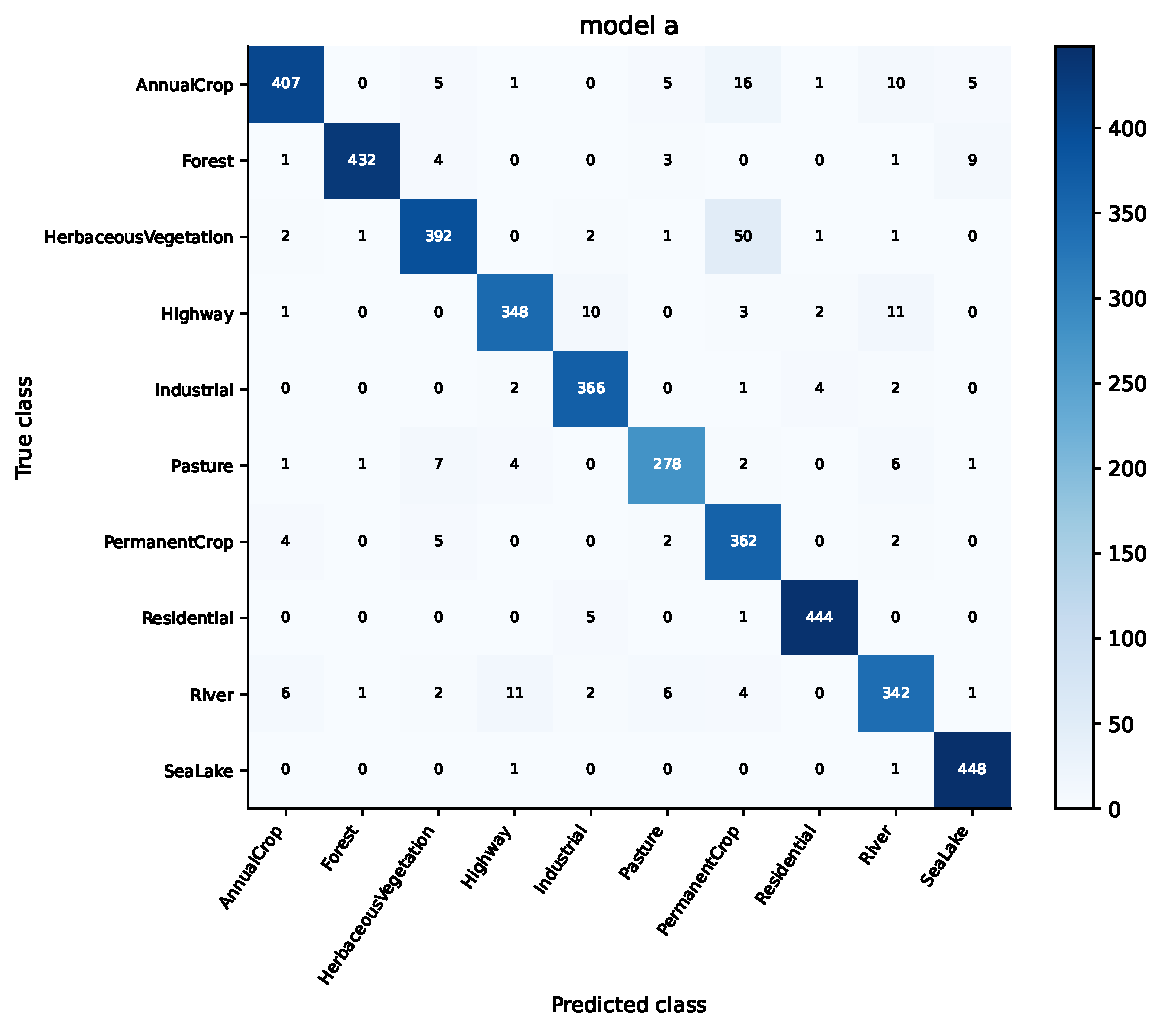
\includegraphics[width=.72\textwidth]{figures/model_a.pdf}
\caption{Model A: numeric counts, true classes on rows and predictions on columns.}
\label{fig:model_a_cm}
\end{figure}
\begin{figure}[H]\centering
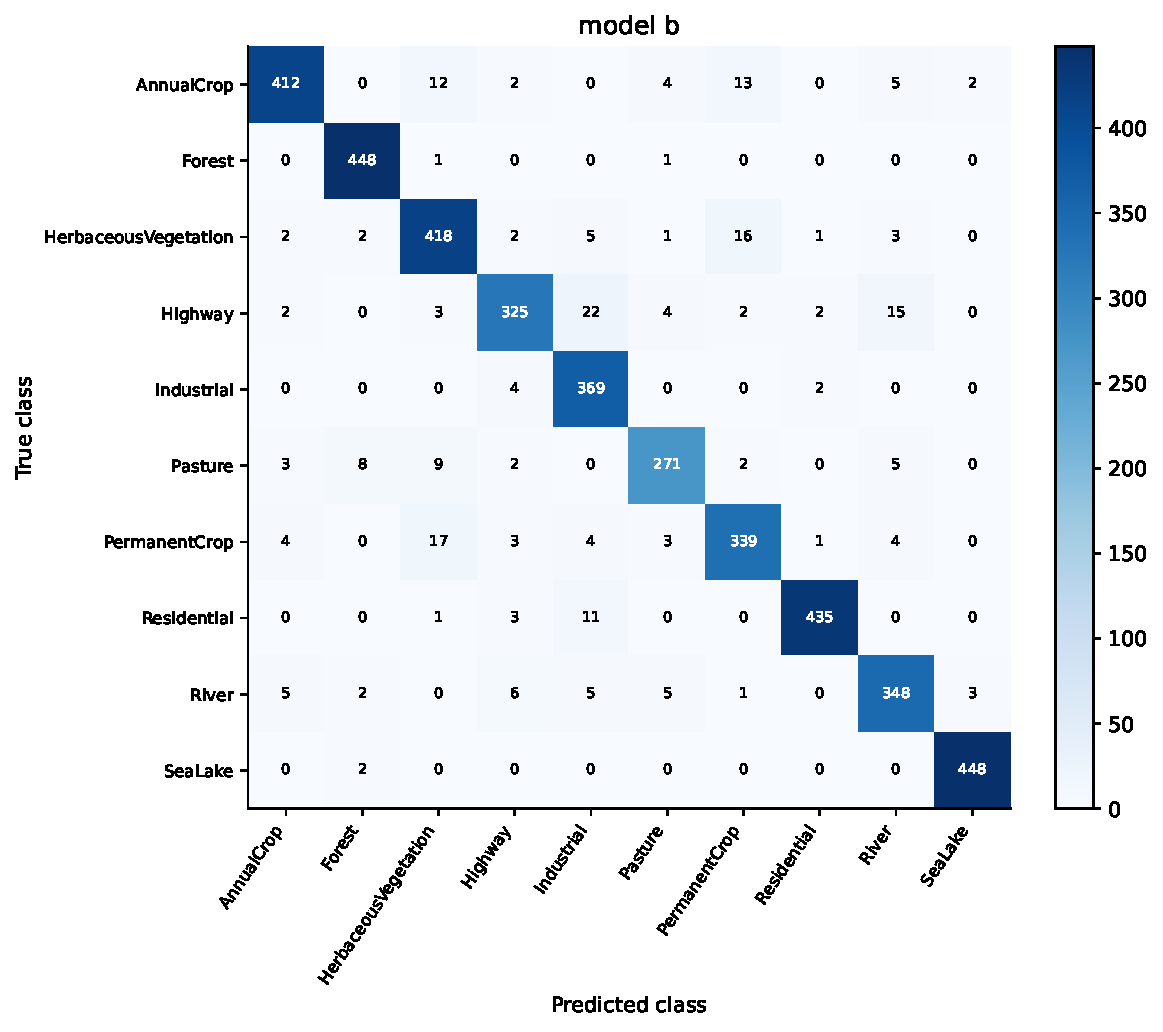
\includegraphics[width=.72\textwidth]{figures/model_b.pdf}
\caption{Model B: numeric counts, true classes on rows and predictions on columns.}
\label{fig:model_b_cm}
\end{figure}
\subsection{Model A vs Model B Resource Comparison}
Table~\ref{tab:custom_resources} compares measured checkpoint sizes and mean
epoch times with parameter and MAC counts. Timing includes training,
validation and batch preprocessing, with CUDA synchronization at the timing
boundaries; it excludes checkpoint and CSV writes. It is therefore a mean
complete-epoch time, not a training-only kernel benchmark.
% Generated from saved experiment evidence; do not edit values.
\begin{table}[H]\centering\small
\caption{Custom-model resources. All parameters are trainable; epoch time includes validation.}\label{tab:custom_resources}
\begin{tabular}{lrrrr}
\toprule
Model & Parameters & Size (KiB) & Epoch (s) & MACs (M) \\ \midrule
Model A & 164,962 & 654.46 & 3.246 & 30.967 \\
Model B & 22,426 & 104.09 & 3.646 & 6.188 \\
\bottomrule
\end{tabular}
\end{table}

Model B reduces whole-network parameters by \ParamReduction\%, serialized
size by \StorageReduction\%, and counted MACs by \MacReduction\%.
Its test accuracy is \CustomAccuracyGap{} percentage points lower. The mean
epoch time nevertheless rises from \AEpochTime{} s to \BEpochTime{} s.
Depthwise kernel efficiency, additional normalization/activation operations
and memory or launch overhead can prevent arithmetic savings from producing
speedups. These are possible explanations; the timing experiment does not
separate their contributions.
